\documentclass[journal,12pt,twocolumn]{IEEEtran}
\usepackage{setspace}
\usepackage[cmex10]{amsmath}
\usepackage{amsthm}
\usepackage{mathrsfs}
\usepackage{enumitem}
\usepackage{mathtools}
\usepackage{graphicx}
\let\vec\mathbf
\title{ASSIGNMENT-1}
\author{CS21BTECH11024 - Varshini  Jonnala}	
\newcommand{\question}{\noindent \textbf{Question: }}
\newcommand{\solution}{\noindent \textbf{Solution: }}
\newcommand{\mydet}[1]{\ensuremath{\begin{vmatrix}#1\end{vmatrix}}}
\newcommand{\myvec}[1]{\ensuremath{\begin{pmatrix}#1\end{pmatrix}}}
\begin{document}
\maketitle
\begin{enumerate}
\item[\textbf{7(c)}]\question $\vec{A}\myvec{2,5}$, $\vec{B}\myvec{-1,2}, \vec{C}\myvec{5,8}$ are the vertices of the triangle $\vec{ABC}$, $\vec{'M'}$ is a point on $\vec{AB}$ such that $AM:MB = 1:2$. Find the co-ordinates of $\vec{'M'}$. Hence find the equation of line passing through the points $\vec{C}$ and $\vec{M}$.
\newline \newline
\solution 
We know that, When the line segment $\vec{AB}$, where the points are $\vec{A}=\myvec{x1\\y1}, \vec{B}=\myvec{x2\\y2}$, is divided internally by $\vec{C}$ in the ratio $m:n$, from Section formula,
 we get the Coordinates of point $\vec{C}$ as,
\begin{align} 
\vec{C} = \myvec{\frac{mx2+nx1}{m+n}\\\\ \frac{my2+ny1}{m+n}},\label{1}
\end{align}
Given, $\vec{M}$ is a point on side $\vec{AB}$ such that $AM:MB = 1:2$. 
Using \eqref{1} in finding $\vec{M}$, we get
\begin{align}
    \vec{M} &= \myvec{\frac{-1+4}{1+2}\\\\ \frac{2+10}{1+2}}\\  \label{3}
   &= \myvec{1\\4}
\end{align}\newline
Let $\vec{L}$ be the line that passes through points $\vec{X,Y}$,Then, $\vec{L}$ can be expressed as
\begin{align}
\label{4}
     \vec{L} &= \vec{X} + \lambda.\hat{XY} ,\\
\hat{XY} &= \frac{\vec{Y} - \vec{X}}{\mydet{\vec{Y} - \vec{X}}} \label{5}
\end{align}

Using \eqref{4} and \eqref{5} to find the equation of the line passing through the points $\vec{C}\myvec{5\\8}$,$\vec{M}\myvec{1\\4}$
\begin{align}
% \hat{CM} &= \frac{\vec{M} - \vec{C}}{\mydet{\vec{M} - \vec{C}}}\\
  \hat{CM} &= \frac{\myvec{5\\8} - \myvec{1\\4}}{\mydet{\myvec{5\\8} - \myvec{1\\4}}}\\
   &= \frac{\myvec{4\\4}}{\mydet{\myvec{4\\4}}}\\
   &= \frac{\myvec{1\\1}}{\sqrt{2}}
\end{align}
The slope of line $\vec{L}$ is $1$.
\\
Thus, Line $\vec{L}$ is $\myvec{1\\4} + \lambda\myvec{1\\1}$. 

 For y-intercept, from the above equation of line $\vec{L}$, it can be written as
 \begin{align}
     \myvec{0\\y} = \myvec{1+\lambda\\4+\lambda} 
 \end{align}
On equating, we get $\lambda$ as $\vec{-1}$, and hence, y-intercept would be $3$.
\\
Thus, the equation of line $\vec{L}$ passing through  $\vec{C}\myvec{5\\8}$ and $\vec{M}\myvec{1\\4}$ is 
\begin{align}
    \myvec{1 & - 1}\vec{x} + 3 &= 0
\end{align}
 which can also be represented as 
 \begin{align}
     x-y+3=0
 \end{align}
 \newpage
{\large But, However,}
We get
\newline
\begin{enumerate}
    \item The equation of the line joining $\vec{A}\myvec{2\\5}, \vec{B}\myvec{-1\\2}$ as $\myvec{1 & - 1}\vec{x} = -3$ and 
    \newline
    \item The equation of the line joining $\vec{B}\myvec{-1\\2}, \vec{C}\myvec{5\\8}$ as $\myvec{1 & - 1}\vec{x}=-3$ too.\newline
\end{enumerate}
 This implies that $\vec{A,B,C}$ points are 'collinear' and lie on the line $\myvec{1 & - 1}\vec{x} = -3$ (or) $x-y+3=0$ and Hence, Given points $\vec{A,B,C}$ don't form a triangle.
\newline
\large Verified by plotting the graph of $\vec{A,B,C}$ and $\vec{M}$ points :

\begin{figure}[ht!]
\centering
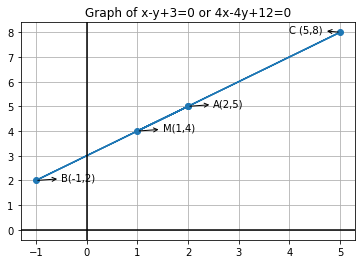
\includegraphics[width=\columnwidth]{prv1.png}
\end{figure}

\end{enumerate}
\end{document}
